\let\negmedspace\undefined
\let\negthickspace\undefined
\documentclass[journal]{IEEEtran}
\usepackage[a5paper, margin=10mm, onecolumn]{geometry}
%\usepackage{lmodern} % Ensure lmodern is loaded for pdflatex
\usepackage{tfrupee} % Include tfrupee package

\setlength{\headheight}{1cm} % Set the height of the header box
\setlength{\headsep}{0mm}     % Set the distance between the header box and the top of the text

\usepackage{gvv-book}
\usepackage{gvv}
\usepackage{cite}
\usepackage{amsmath,amssymb,amsfonts,amsthm}
\usepackage{algorithmic}
\usepackage{graphicx}
\usepackage{textcomp}
\usepackage{xcolor}
\usepackage{txfonts}
\usepackage{listings}
\usepackage{enumitem}
\usepackage{mathtools}
\usepackage{gensymb}
\usepackage{comment}
\usepackage[breaklinks=true]{hyperref}
\usepackage{tkz-euclide} 
\usepackage{listings}
% \usepackage{gvv}                                        
\def\inputGnumericTable{}                                 
\usepackage[latin1]{inputenc}                                
\usepackage{color}                                            
\usepackage{array}                                            
\usepackage{longtable}                                       
\usepackage{calc}                                             
\usepackage{multirow}                                         
\usepackage{hhline}                                           
\usepackage{ifthen}                                           
\usepackage{lscape}
\begin{document}

\bibliographystyle{IEEEtran}
\vspace{3cm}

\title{9.2.1}
\author{EE24BTECH11012 - Bhavanisankar G S}
% \maketitle
% \newpage
% \bigskip
{\let\newpage\relax\maketitle}

\renewcommand{\thefigure}{\theenumi}
\renewcommand{\thetable}{\theenumi}
\setlength{\intextsep}{10pt} % Space between text and floats


\numberwithin{equation}{enumi}
\numberwithin{figure}{enumi}
\renewcommand{\thetable}{\theenumi}

\textbf{LAPLACE TRANSFORMS} \\
\begin{itemize}
	%\item Transformation applied on a function results in a function of another variable, unlike an operation which when applied on a function yields another function but of the same variable.
	%\item Laplace transform is a very useful technique used to solve complex equations using \textbf{integral transformations}.
	%\item Any equation of the form $\int_{a}^{b} f(t) K(p,t) dt = F(p)$ is called an integral transformation, and the function $K(p,t)$ is called the \textbf{Kernel function}. \\
		%When $a = 0 \text{ and } b = \infty$, then the integral transformation is called the Laplace transformation.
	\item \textbf{Notation} : Laplace transform of a function $f(x)$ is denoted as $\mathcal{L} \brak{f(x)}$, i.e., 
		\begin{align}
			\mathcal{L} \brak{f(x)} = F(s) = \int_{0}^{\infty} f(x) e^{-sx} dx \label{eq:lap} 
		\end{align}
	\item It is a linear transformation, since integration is a linear operation.
	\item \textbf{Laplace transform of some functions :} 
		\begin{align}
			f(x) = 0 &\implies F(s) = 0 \\
			f(x) = 1 &\implies F(s) = \frac{1}{s} \text{ for } Re(s) > 0\\
			f(x) = x^n &\implies F(s) = \frac{n!}{s^{n+1}} \text{ for } Re(s) > 0 \\
			f(x) = e^{at} &\implies F(s) = \frac{1}{s-a} \text{ for } Re(s) > a \\
			f(x) = \sin{ax} &\implies F(s) = \frac{a}{s^2 + a^2} \text{ for } Re(s) > 0 \\
			f(x) = \cos{ax} &\implies F(s) = \frac{s}{s^2 + a^2} \text{ for } Re(s) > 0
		\end{align}
	\item \textbf{Some other useful results include :}
		\begin{align}
			\mathcal{L} \brak{f^{\prime}(x)} &= s F(s) - f(0^{-}) \\
			\mathcal{L} \brak{f^{\prime \prime}(x)} &= s^2 F(s) - s f(0^{-}) - f^{\prime}(0^{-}) 
		\end{align}
	\item \textbf{Laplace transform of unit step function $u(t)$ :} \\
		\begin{align}
			u(t) &= 
			\begin{cases} 
			1 & t \geq 0 \\
			0 & t < 0
			\end{cases} \label{eq:ut}
		\end{align}
			\text{From \eqref{eq:lap}}
		\begin{align}
			\mathcal{L} \brak{u(t)} &= \int_{0}^{\infty} u(t) e^{-st} dt 
		\end{align}
		For all non-negative values, $u(t) = 1$. Hence, the integral becomes,
		\begin{align}
			F(s) &= \int_{0}^{\infty} (1)e^{-st} dt \\
			F(s) &= \left[ \frac{e^{-st}}{-s} \right]_{0}^{\infty} = \frac{1}{s} ,  \text{ for } Re(s) > 0 \label{eq:first}
		\end{align}
	\item \textbf{Laplace transform of $e^{at} u(t)$ :} \\
		From \eqref{eq:lap}
		\begin{align}
			\mathcal{L} \brak{e^{at} u(t)} &= \int_{0}^{\infty} e^{at} u(t) e^{-st} dt \\
			F(s) &= \int_{0}^{\infty} e^{(a-s)t} dt \\
			F(s) &= \left[\frac{e^{(a-s)t}}{a-s} \right]_{0}^{\infty} = \frac{1}{s-a} , \text{ for } Re(s) > a
		\end{align}
		When $a=1$, 
		\begin{align}
			F(s) = \mathcal{L} \brak{e^t u(t)} = \frac{1}{s-1} \label{eq:second} \text{ for } Re(s) > 1  
		\end{align}
\end{itemize}

\textbf{Z-TRANSFORMS} 
\begin{itemize}
	\item \textbf{Notation} : 
		\begin{align}
			Y(z) &= \sum_{n \to -\infty}^{\infty} y_{n} z^{-n} \label{eq:z}
		\end{align}
	\item \textbf{Z-transform of $u(t)$} : \\
		From \eqref{eq:z}
		\begin{align}
			Y(z) &= \sum_{t \to -\infty}^{\infty} u(t) z^{-t} 
		\end{align}
		From \eqref{eq:ut}, this can be simplified to
		\begin{align}
		        Y(z) &= \sum_{t=0}^{\infty} (1)z^{-t} \\
			Y(z) &= \frac{1}{1 - z^{-1}}, \label{eq:zut} \text{ for } \abs{z} > 1 
		\end{align}
	\item \textbf{Z-transform of $a^t u(t)$} : \\
		From \eqref{eq:z} 
		\begin{align}
			Y(z) &= \sum_{t \to -\infty}^{\infty} a^t u(t) z^{-t} 
		\end{align}
		From \eqref{eq:ut}, this can be simplified to
		\begin{align}
			Y(z) &= \sum_{t=0}^{\infty} a^t z^{-t} \\
			Y(z) &= \sum_{t=0}^{\infty} \brak{az^{-1}}^{t} \\
			Y(z) &= \frac{1}{1 - az^{-1}}, \text{ for } \abs{z} > \abs{a} \label{eq:atut}
		\end{align}
	\item \textbf{Some other useful results} : \\
		\begin{align}
			Y(u_{n-1}) &= z^{-1} Y(u_{n}) \\
			Y(u_{n+1}) &= z \brak{Y(u_{n}) - u_{0}}
		\end{align}
\end{itemize}


\textbf{QUESTION}:\\
Consider the differential equation $\frac{d^2 y}{d x^2} - \frac{dy}{dx} = 0$. Verify that $y = e^x + 1$ is a solution for it, given the initial condtitions $y(0) = 2 \text{ and } y^{\prime} (0) = 1$ . \\
\textbf{SOLUTION}: \\
%\input{tables/table.tex} \\ \\ \\
Consider the differential equation, 
\begin{align} 
	\frac{d^2 y}{d x^2} - \frac{dy}{dx} = 0 \label{eq:third} 
\end{align}
Integrating \eqref{eq:third} on both the sides, we have, 
\begin{align}
	\int \brak{\frac{d^2 y}{d x^2} - \frac{dy}{dx}} dx &= \int \brak{0} dx \\
	\frac{dy}{dx} - y &= k  
\end{align}
where, $k$ is a constant. Applying the initial conditions, we have
\begin{align}
	k &= 1-2 = -1 \\
	\frac{dy}{dx} &= y - 1 \label{eq:fourth}
\end{align}
Applying Laplace transform to \eqref{eq:third} on both sides, we have \\
\begin{align}
	\mathcal{L} \brak{\frac{d^2 y}{d x^2} - \frac{dy}{dx}} &= \mathcal{L} \brak{0} \\
	\mathcal{L} \brak{\frac{d^2 y}{d x^2}} - \mathcal{L} \brak{\frac{dy}{dx}} &= \mathcal{L} \brak{0} \\
	\brak{s^2 F(s) - s f(0^{-}) - f^{\prime}(0^{-})} - \brak{s F(s) - f(0^{-})} &= 0 \\
	F(s) \brak{s^2 - s} - f(0^{-}) \brak{s-1} - f^{\prime}(0^{-}) &= 0 \\
	F(s) &= \frac{f(0^{-}) \brak{s-1} + f^{\prime}(0^{-})}{s^2 - s} \\
	\mathcal{L} \brak{f(x)} &= \frac{f(0^{-}) - f^{\prime}(0^{-})}{s} + \frac{f^{\prime}(0^{-})}{s-1}  
\end{align} \\
Substituting the initial conditions, $y(0^{-}) = 2 \text{ and } y^{\prime} (0^{-}) = 1$, we have \\ 
\begin{align}
	f(x) &= \mathcal{L}^{-1} \brak{\frac{1}{s} + \frac{1}{s-1}} \\
	f(x) &= \mathcal{L}^{-1} \brak{\frac{1}{s}} + \mathcal{L}^{-1} \brak{\frac{1}{s-1}}  
\end{align}
From, \eqref{eq:first} and \eqref{eq:second}, it can be deduced that
\begin{align}
	f(x) &= u(x) + e^x u(x) \\
	&= u(x) \brak{1 + e^x}
\end{align}
Hence, verified. \\
\textbf{ALGORITHM :} \\
\begin{align}
	 x_0 &= 0 \\
	 y_0 &= 2 \\
	 h &= 0.01 \\
	 x_{n+1} &= x_{n} + h \\
	 y_{n+1} &= y_{n} + h \brak{y^{\prime}} 
\end{align}
From \eqref{eq:fourth}, 
\begin{align}
	y_{n+1} &= y_{n} + h \brak{y_{n} - 1} \label{eq:difeq}
\end{align}
which is the required difference equation. \\
Applying unilateral ( one-sided ) z-transform on both sides of \eqref{eq:difeq}, we have
\begin{align}
	Y(y_{n+1}) &= Y(y_{n} \brak{1+h} - h) \\
	z Y(z) - z y_{0} &= (1+h) Y(z) - h \frac{1}{1 - z^{-1}} \\
	Y(z) \brak{z - (1+h)} &= z y_{0} - \frac{h}{1 - z^{-1}} 
\end{align}
Substituting $y_{0} = 2$ and simplifying, we have
\begin{align}
	Y(z) &= \frac{1}{1 - \brak{1+h} z^{-1}} + \frac{1}{1 - z^{-1}}
\end{align}
From \eqref{eq:zut} and \eqref{eq:atut}, applying Inverse-Z-Transform on both sides, we have 
\begin{align}
	y_{n} &= \brak{1+h}^{n} u(n) + (1) u(n)	\\
	 &= u(n) \brak{1 + \brak{1+h}^{n}} \label{eq:ans}
\end{align}
The plot corresponding to \eqref{eq:ans} is given below.

\begin{figure}[h]
				 \centering
				 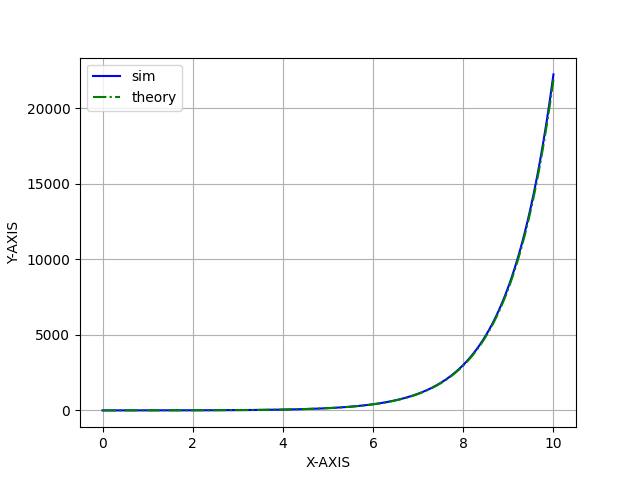
\includegraphics[width=\columnwidth]{figs/fig.png}
				 \caption{A plot of the given question.}
				 \label{fig:Plot1}
			 \end{figure}


\end{document}
